\documentclass{article}

\usepackage{graphicx} % Required for inserting images
\usepackage[T1]{fontenc}
\usepackage[utf8]{inputenc}
\usepackage[english]{babel}
\usepackage{listings}
\usepackage{xcolor}
\sloppy 

\lstdefinestyle{javaStyle}{
    language=Java,
    basicstyle=\ttfamily\footnotesize, % Czcionka kodu
    keywordstyle=\color{blue},         % Kolor słów kluczowych
    commentstyle=\color{gray},         % Kolor komentarzy
    stringstyle=\color{red},           % Kolor stringów
    numbers=left,                      % Numery wierszy
    numberstyle=\tiny\color{gray},     % Styl numerów wierszy
    stepnumber=1,                      % Numer co każdy wiersz
    breaklines=true,                   % Łamanie długich linii
    tabsize=4                          % Wielkość tabulacji
}
\lstset{
    breaklines=true,      % Łamanie długich linii
    breakatwhitespace=true, % Łamanie tylko w miejscach białych znaków
    columns=fullflexible, % Pozwala na dynamiczne dostosowanie szerokości
    basicstyle=\ttfamily\footnotesize % Mniejsza czcionka
}

\title{Dokumentacja Projektu Bazy danych 2 \\ \large Inwentaryzacja Sprzętu SKN MOS }

\author{Jakub Maciocha nr. albumu 272949 \and Kornel Uriasz nr. albumu 272967 \and Maciej Pacholczyk nr. albumu 272873}
\date{Październik 2024}

\begin{document}

\maketitle

\newpage
\section{\textbf{ETAP I - Opis świata rzeczywistego}}
    \subsection{Kontekst bieżący}
    Studenckie koło naukowego Microsystem Oriented Society (SKN MOS) prowadzi inwentaryzacje oraz możliwość wypożyczania sprzętu oraz narzędzi dla członków grupy w ramach działania koła naukowego. Siedziba koła zlokalizowana jest w podpiwniczeniu akademika T4 "Czworak", gdzie magazynowany jest sprzęt. Działanie opiera się na rejestrowaniu oraz monitorowaniu sprzętu oraz narzędzi przez administratorów koła naukowego. W tym przypadku są to członkowie zarządu. Katalogują oraz przechowując wszystkie informacje, które są im niezbędne do poprawnego działania koła oraz działania w ramach instytucji Politechniki Wrocławskiej. Taki system w bieżącym momencie pozwala w łatwy sposób zarządzać dostępnymi zasobami.

    \subsection{Opis zasobów ludzkich oraz procesów}
    Proces inwentaryzacji, na moment definiowania nowego systemu, opiera się na fizycznym odnotowywaniu nowego sprzętu z wykorzystanie numerów id lub jego nazwy. Archiwizacja urządzeń odbywa się w formie papierowej, na papierowym arkuszu. Spis sprzętów wypożyczonych prowadzony jest w oddzielnych zasobach w postaci listy  wypożyczeń. Lista ta jest przechowywana również na arkuszu papieru. Proces inwentaryzacji musi być jawny dla klienta jak i dla administratora tj. Klient zobowiązany jest do wiedzy na temat przedmiotu wypożyczenia oraz terminu jego zwrotu. Administrator natomiast powinien dysponować przejrzystą listą, zawierającą informacje o tym, kto, co wypożyczył oraz do kiedy ma obowiązek zwrócić dany przedmiot. Nie może zaistnieć sytuacja, w której administrator nie posiada wiedzy o lokalizacji wypożyczonego przedmiotu, ani sytuacja, w której klient nie jest świadomy, co zostało wypożyczone i w jakim terminie ma obowiązek zwrotu.    
    Inwentaryzacja w bieżącym momencie jest prosta, intuicyjna oraz łatwa do przyswojenia dla nowych członków koła, którzy systematycznie dołączają. Proces jest jednak mało wydajny przy zwiększającej się liczbie sprzętu oraz członków koła naukowego. Wzrost ilości dokumentacji dot. sprzętu oraz jego wypożyczeń skutkuje brakiem przejrzystości, trudnościami w archiwizacji oraz lokalizacją sprzętu. Podsumowując proces jest czasochłonny oraz podatny na błędy systemowe.

    W bieżącym momencie osoby działające w obrębie sytemu można podzielić na dwie grupy użytkowników. Pierwsza grupa to użytkownicy z uprawnieniami do odczytu. Klasyfikują się do niej członkowie koła, którzy mogą w swobodny sposób korzystać oraz wypożyczać sprzęt z placówki koła naukowego. W tym momencie do przedstawianego zbioru należy około \textbf{30} członków koła. Druga grupa użytkowników to administratorzy dbający o archiwizację oraz posiadający uprawnienia do wypożyczania sprzętu. Osoby
    te monitorują dostępne zasoby w kole naukowym oraz dbają o przechowywanie dokumentów potwierdzających stan odpowiednich przedmiotów. Do wymienionej grupy należy od \textbf{5 do 10} członków zarządu, którzy stają się administratorami. \newline
    Liczba administratorow : \textbf{5 - 10} \newline
    Liczba klientow : \textbf{30}
    
\section{\textbf{ETAP II}}
    \subsection{Wymagania funkcjonalne i niefunkcjonalne}
    Klient (administratorzy) przedstawili następne funkcjonalności dla systemu usprawniającego proces inwentaryzacji oraz wypożyczeń.
        \begin{enumerate}
            \item Funkcjonalne
            
            \begin{enumerate}
                \item Aplikacja przedluża okres wypożyczenia na życzenie klienta, po zatwierdzeniu przez administratora
                \item Aplikacja ponagla o oddanie przedmiotu na zapytanie administratora
                \item Aplikacja decyduje o prawidłowym/nieprawidłowym oddaniu przedmiotu na podstawie daty wypożyczenia oraz aktualnej daty
                \item Aplikacja pokazuje przefiltrowane dane na żądanie klienta
                \item Aplikacja weryfikuje uprawnienia klienta
                \item Aplikacja wysyła powiadomienia o upływającym terminie wypożyczeń
                \item Aplikacja generuje miesięczne raporty sprzętowe
            \end{enumerate}

            \item Niefunkcjonalne 

            \begin{enumerate}
                \item Lokalizacja serwera w pokoju socjalnym w siedzibie koła naukowego
                \item Strona posiada przejrzysty interfejs
                \item Strona jest atrakcyjna/estetyczna
                \item Aplikacja jest umieszczona na serwerze koła naukowego
                \item Aplikacja przestrzega obostrzeń RODO
            \end{enumerate}
            
        \end{enumerate}

Diagram przypadkow uzycnia

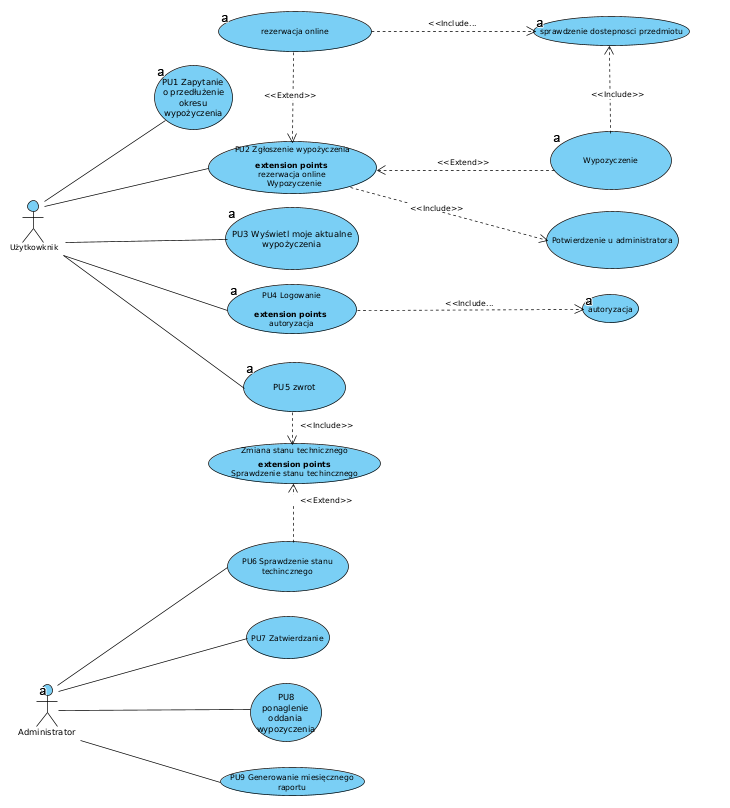
\includegraphics[width=\textwidth]{media/use_case.png}
\subsection{PU1: Rezerwacja}

\subsubsection{Cel}
Umożliwienie użytkownikowi zarezerwowania przedmiotu dostępnego w systemie na wybrany okres.

\subsubsection{Aktorzy}
\begin{itemize}
    \item \textbf{Użytkownik} - osoba korzystająca z systemu, która chce zarezerwować przedmiot.
\end{itemize}

\subsubsection{Zdarzenie inicjujące}
Użytkownik chce zarezerwować przedmiot, aby mieć pewność, że będzie on dostępny w określonym czasie.

\subsubsection{Warunki wstępne}
Użytkownik jest zalogowany do systemu i przedmiot, który chce zarezerwować, jest dostępny do rezerwacji.

\subsubsection{Warunki końcowe (wyniki)}
\begin{itemize}
    \item \textbf{Sukces:} Przedmiot jest zarezerwowany dla użytkownika na określony okres.
    \item \textbf{Niepowodzenie:} Użytkownik otrzymuje informację, że rezerwacja nie jest możliwa, ponieważ przedmiot nie jest dostępny.
\end{itemize}

\subsubsection{Scenariusz główny}
\begin{enumerate}
    \item Użytkownik loguje się do systemu.
    \item Użytkownik wybiera opcję „Rezerwacja” i przegląda dostępne przedmioty.
    \item Użytkownik wybiera przedmiot i określa termin, na który chce go zarezerwować.
    \item System sprawdza dostępność przedmiotu w wybranym terminie.
    \item Jeśli przedmiot jest dostępny, system rejestruje rezerwację.
    \item Użytkownik otrzymuje potwierdzenie rezerwacji.
\end{enumerate}

% Przypadek użycia 2: Wypożyczenie
\subsection{PU2: Wypożyczenie}

\subsubsection{Cel}
Umożliwienie użytkownikowi wypożyczenia przedmiotu na określony czas.

\subsubsection{Aktorzy}
\begin{itemize}
    \item \textbf{Użytkownik} - osoba korzystająca z systemu, która chce wypożyczyć przedmiot.
    \item \textbf{Administrator} - osoba odpowiedzialna za potwierdzenie wypożyczenia.
\end{itemize}

\subsubsection{Zdarzenie inicjujące}
Użytkownik chce wypożyczyć przedmiot na określony czas.

\subsubsection{Warunki wstępne}
Użytkownik jest zalogowany do systemu i przedmiot, który chce wypożyczyć, jest dostępny.

\subsubsection{Warunki końcowe (wyniki)}
\begin{itemize}
    \item \textbf{Sukces:} Przedmiot zostaje wypożyczony na rzecz użytkownika.
    \item \textbf{Niepowodzenie:} Użytkownik otrzymuje informację, że wypożyczenie nie jest możliwe (np. z powodu niedostępności przedmiotu).
\end{itemize}

\subsubsection{Scenariusz główny}
\begin{enumerate}
    \item Użytkownik loguje się do systemu.
    \item Użytkownik wybiera opcję „Wypożyczenie” i przegląda dostępne przedmioty.
    \item Użytkownik wybiera przedmiot do wypożyczenia i określa czas wypożyczenia.
    \item System sprawdza, czy przedmiot jest dostępny w wybranym czasie.
    \item Użytkownik potwierdza wypożyczenie.
    \item System przesyła prośbę do Administratora o potwierdzenie wypożyczenia.
    \item Administrator zatwierdza lub odrzuca wypożyczenie.
    \item Użytkownik otrzymuje informację o decyzji Administratora.
\end{enumerate}

% Przypadek użycia 3: Zwrot
\subsection{PU3: Zwrot}

\subsubsection{Cel}
Umożliwienie użytkownikowi zwrócenia wypożyczonego przedmiotu po zakończeniu okresu wypożyczenia.

\subsubsection{Aktorzy}
\begin{itemize}
    \item \textbf{Użytkownik} - osoba korzystająca z systemu, która chce zwrócić przedmiot.
    \item \textbf{Administrator} - osoba odpowiedzialna za sprawdzenie stanu technicznego zwróconego przedmiotu.
\end{itemize}

\subsubsection{Zdarzenie inicjujące}
Użytkownik kończy korzystanie z przedmiotu i chce go zwrócić.

\subsubsection{Warunki wstępne}
Użytkownik jest zalogowany do systemu i posiada wypożyczony przedmiot, który chce zwrócić.

\subsubsection{Warunki końcowe (wyniki)}
\begin{itemize}
    \item \textbf{Sukces:} Przedmiot zostaje zwrócony, a system aktualizuje jego stan jako dostępny.
    \item \textbf{Niepowodzenie:} Zwrot nie zostaje zrealizowany z powodu błędu w systemie lub problemu z przedmiotem.
\end{itemize}

\subsubsection{Scenariusz główny}
\begin{enumerate}
    \item Użytkownik loguje się do systemu.
    \item Użytkownik wybiera opcję „Zwrot” i wybiera przedmiot, który chce zwrócić.
    \item Użytkownik potwierdza zwrot przedmiotu.
    \item System rejestruje próbę zwrotu i informuje Administratora.
    \item Administrator sprawdza stan techniczny przedmiotu.
    \item Jeśli przedmiot jest w dobrym stanie, Administrator zatwierdza zwrot.
    \item System aktualizuje stan przedmiotu jako dostępny.
    \item Użytkownik otrzymuje potwierdzenie pomyślnego zwrotu.
\end{enumerate}

\section{\textbf{ETAP III}}

\subsection{\textbf{Diagramy ERD}}
  \begin{itemize}
    \item Konceptualny 
          Diagram konceptualny ERD (z ang. Entity-Relationship Diagram) przedstawia ogólną strukturę bazy danych, bez wnikania w szczegóły techniczne. Skupia się na identyfikacji kluczowych encji i ich relacji, aby zrozumieć, jakie informacje będą przechowywane w bazie i jak poszczególne elementy będą się ze sobą łączyć. Zostały w nim przedstawione tabele dostępne w systemie, relacje pomiędzy tabelami oraz kolumny zaiwerające klucz główny dla tabeli.   
    
    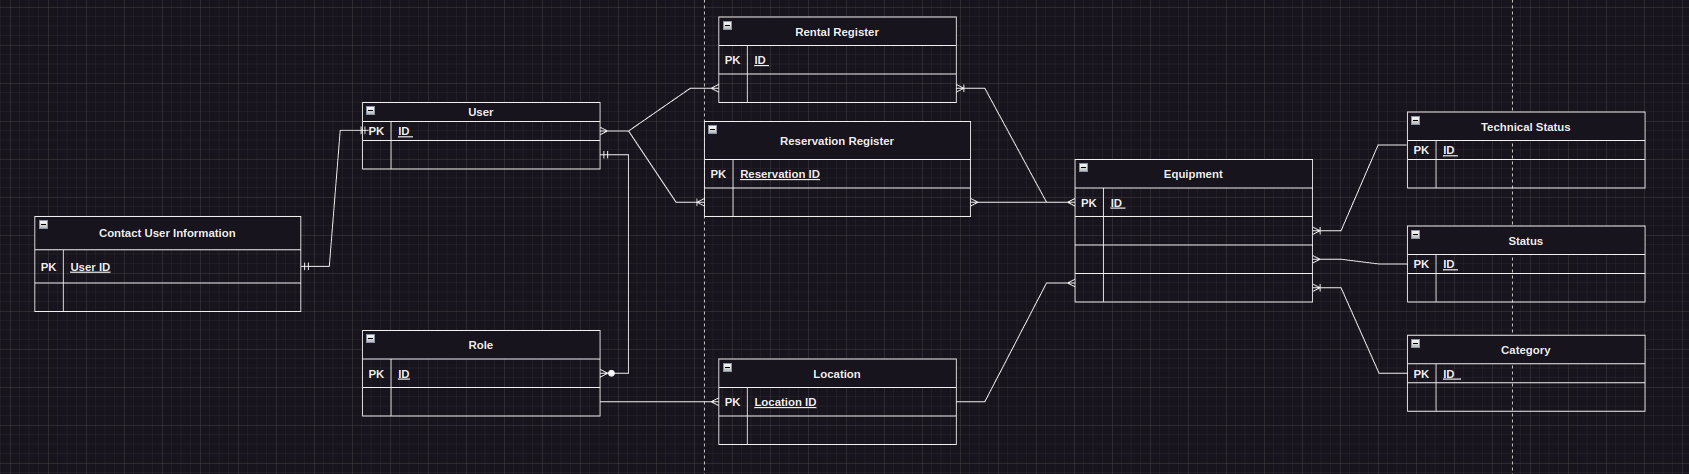
\includegraphics[width=\textwidth]{media/conceptual_erd.png}

    \item Logiczny
          Diagram logiczny ERD rozszerza konceptualny model danych, dodając szczegóły na temat struktur encji. Na tym etapie diagram przedstawia już kolumny z nazwami. Diagram logiczny pokazuje też typy relacji między encjami, w tym relacje wiele-do-wielu, jednak nadal pomija szczegóły techniczne związane z fizycznym implementowaniem bazy danych. Na diagramie pojawia się również typy kolumn w formie ogólnej, ale są one jeszcze niezwiązane z konkretnym silnikiem bazy danych.

     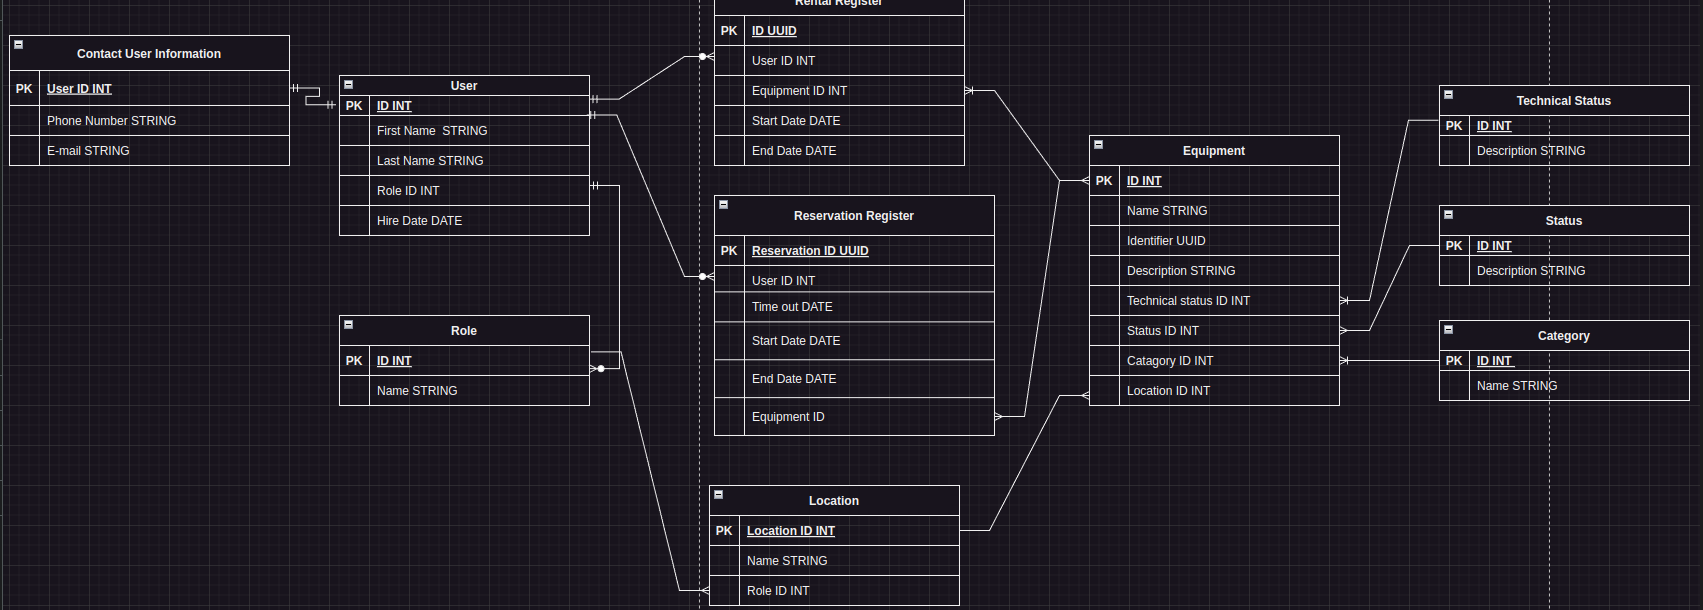
\includegraphics[width=\textwidth]{media/logical_erd.png}

    \item Fizyczny
        Diagram fizyczny ERD jest ostatecznym, szczegółowym modelem bazy danych, który uwzględnia wszystkie techniczne aspekty jej implementacji. Ten diagram zawiera wszystkie encje, kolumny oraz szczegółowe typy danych zgodne z wymaganiami wybranego silnika bazy danych. Nazwy encji i kolumn są dostosowane tak, aby były zgodne z konwencjami bazy danych (bez spacji i niedozwolonych znaków). Fizyczny ERD przedstawia także klucze główne oraz obce, a także rozwiązane relacje wiele-do-wielu, które są realizowane przez tabele pośredniczące. Diagram zwiera również  wyzwalacze (triggers) oraz inne mechanizmy logiczne potrzebne do poprawnego działania bazy danych.

      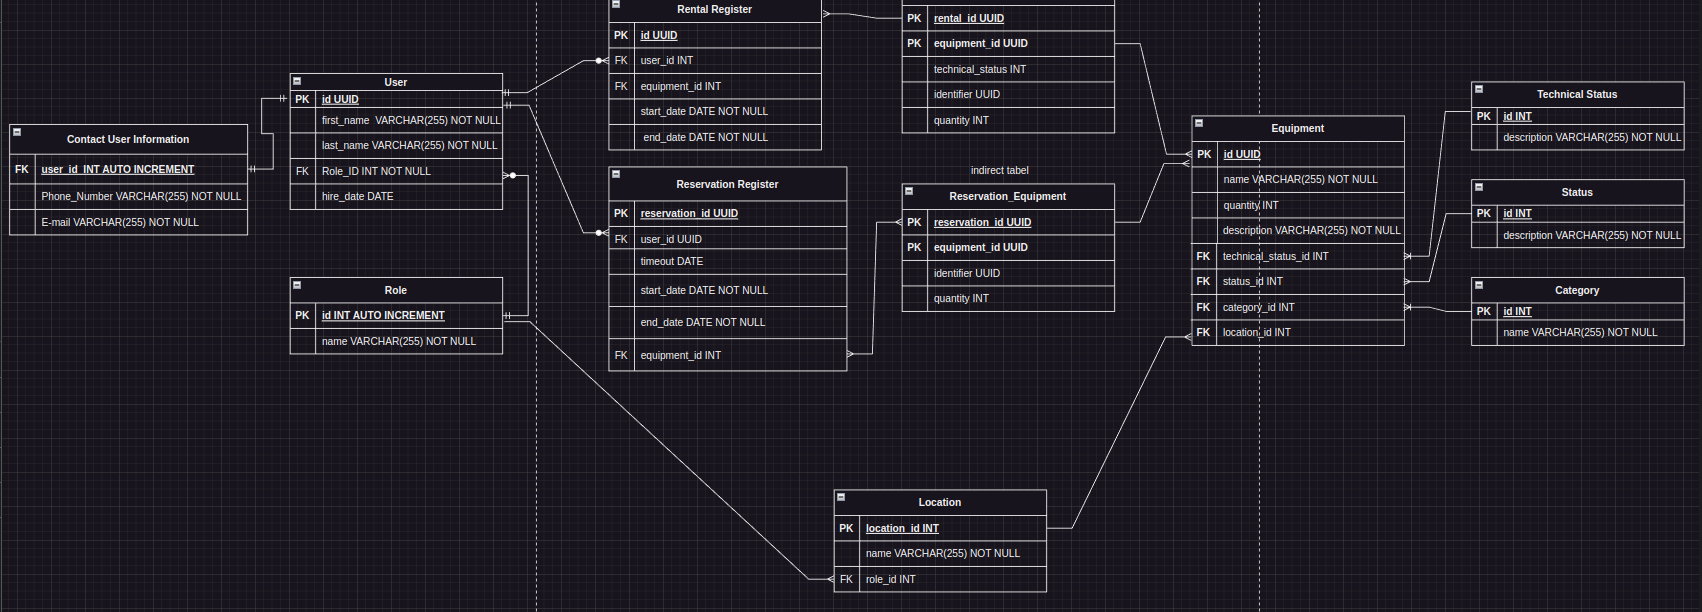
\includegraphics[width=\textwidth]{media/physical_erd.png}

  \end{itemize}

\subsection{\textbf{Analiza wielkości tabel i częstości odwołań do tabel i kolumn}}

Zakładając, że w systemie mamy \textbf{200 unikalnych przedmiotów (sprzętu)} oraz że liczba wypożyczeń wynosi \textbf{5 wypożyczeń tygodniowo}, poniżej przedstawiona jest analiza liczby rekordów w tabelach oraz częstości odwołań do tabel i kolumn.

\subsubsection{Liczność rekordów w tabelach}
Zakładając 5 wypożyczeń tygodniowo i średnio 2 przedmioty na wypożyczenie, liczba rekordów w tabelach wygląda następująco:

\begin{table}[h!]
    \centering
        \begin{tabular}{|l|l|l|}
            \hline
            \textbf{Tabela} & \textbf{Opis}  & \textbf{Liczba rekordów} \\ \hline
            Rental\_register & Rejestr wypożyczeń & 260 wypożyczeń rocznie \\ \hline
            Equipment & Lista sprzętu(200 unikalnych przedmiotów) & 200 rekordów \\ \hline
            Rental\_Equipment & Powiązania sprzętu z wypożyczeniami & 500 powiązań rocznie \\ \hline
        \end{tabular}
    \caption{Liczność rekordów w tabelach}
\end{table}

\subsubsection{\textbf{Częstość odwołań do tabel i kolumn}}
Poniżej przedstawiono przewidywaną częstość odwołań do tabel i kolumn na podstawie liczby operacji w systemie.

\begin{table}[h]
    \centering
        \begin{tabular}[width=\textwidth]{|l|l|p{5cm}|l|}
            \hline
            \textbf{Tabela} & \textbf{Operacja} & \textbf{Opis} & \textbf{Częstość} \\ \hline
            Rental\_register& INSERT  & Dodawanie nowych wypożyczeń. & Niska  \\ \hline
             ~ & SELECT & Pobieranie historii wypożyczeń użytkowników. & Średnia. \\ \hline
             ~ & UPDATE & Aktualizacja dat zakończenia wypożyczeń lub innych danych. & Niska \\ \hline
            Equipment & SELECT & Pobieranie listy sprzętu. & Wysoka  \\ \hline
              & UPDATE & Zmiana statusu sprzętu. & Średnia \\ \hline
            Rental\_Equipment & SELECT & Pobieranie sprzętu dla danego wypożyczenia. & Średnia \\ \hline
              & INSERT & Dodawanie powiązań między wypożyczeniem a sprzętem. & Niska \\ \hline
        \end{tabular}
    \caption{Częstość odwołań do tabel i kolumn}
\end{table}

\subsubsection{Propozycje indeksów}
W celu optymalizacji zapytań, zwłaszcza dla tabel, które będą miały dużą liczbę operacji odczytu, zaproponowane indeksy wyglądają następująco:

\begin{itemize}
    \item \textbf{Tabela `Rental\_register`}: 
    \begin{itemize}
        \item \textbf{Primary Key:} `id` – identyfikator wypożyczenia.
        \item \textbf{Indeks:} `user\_id` – przyspiesza wyszukiwanie wypożyczeń dla konkretnego użytkownika.
        \item \textbf{Indeks:} `(start\_date, end\_date)` – ułatwia filtrowanie wypożyczeń w zadanym zakresie dat.
        \item \textbf{Indeks:} `equipment\_id` – umożliwia szybkie wyszukiwanie powiązań z poszczególnymi przedmiotami.
    \end{itemize}
    
    \item \textbf{Tabela `Equipment`}: 
    \begin{itemize}
        \item \textbf{Primary Key:} `id` – identyfikator sprzętu.
        \item \textbf{Indeks:} `status` – przyspiesza filtrowanie sprzętu według jego statusu (`available`, `rented`).
        \item \textbf{Indeks:} `category\_id` – przyspiesza filtrowanie sprzętu według kategorii.
    \end{itemize}
    
    \item \textbf{Tabela `Rental\_Equipment`}: 
    \begin{itemize}
        \item \textbf{Composite Primary Key:} `(rental\_id, equipment\_id)` – pozwala szybko łączyć dane z tabeli `Rental\_register` i `Equipment`.
        \item \textbf{Indeks:} `equipment\_id` – umożliwia szybkie wyszukiwanie sprzętu wypożyczonego w ramach danego wypożyczenia.
    \end{itemize}
\end{itemize}

\subsubsection{\textbf {Przykłady zapytań i ich optymalizacja}}

Poniżej przedstawiono przykłady zapytań oraz optymalizacje na podstawie proponowanych indeksów:

\begin{itemize}
    \item \textbf{Wyszukiwanie historii wypożyczeń użytkownika:}
    \begin{verbatim}
    SELECT * 
    FROM Rental_register 
    WHERE user_id = 123 
    ORDER BY start_date DESC;
    \end{verbatim}
    Indeks: `user\_id` oraz `(user\_id, start\_date)`.

    \item \textbf{Pobieranie dostępnego sprzętu w danej kategorii:}
    \begin{verbatim}
    SELECT * 
    FROM Equipment 
    WHERE status = 'available' AND category_id = 3;
    \end{verbatim}
    Indeks: `(status, category\_id)`.

    \item \textbf{Pobieranie sprzętu wypożyczonego w ramach danego wypożyczenia:}
    \begin{verbatim}
    SELECT e.name, e.description
    FROM Rental_Equipment re
    JOIN Equipment e ON re.equipment_id = e.id
    WHERE re.rental_id = 456;
    \end{verbatim}
    Indeks: `(rental\_id, equipment\_id)` w tabeli `Rental\_Equipment`.
\end{itemize}

\subsubsection{Podsumowanie}
Zmniejszenie liczby unikalnych przedmiotów (200 unikalnych przedmiotów) nie zmienia istotnie analizowanej struktury, jednak wpływa na zapytania przetwarzające dane o sprzęcie. Dla tabeli \texttt{Equipment}, która zawiera 200 rekordów, konieczne jest zastosowanie indeksów na kolumnach takich jak \texttt{status}, \texttt{category\_id} czy \texttt{id}, aby przyspieszyć operacje odczytu. Proponowane indeksy dla tabel \texttt{Rental\_register} i \texttt{Rental\_Equipment} powinny również zoptymalizować operacje wyszukiwania powiązań między wypożyczeniami a sprzętem.

Zoptymalizowane zapytania oraz odpowiednio zaplanowane indeksy zapewnią płynność działania systemu, nawet przy większej liczbie operacji odczytu i zapisu, co jest szczególnie istotne dla użytkowników oraz administratorów systemu.

\subsection{Analiza Integralności Danych}

Aby zapewnić integralność danych na podstawie dostarczonego diagramu ERD, analizujemy kluczowe zależności i relacje między tabelami. W poniższej tabeli przedstawiono rekomendowane akcje ``cascade delete'' lub wyzwalacze, które należy zastosować:

\begin{table}[h]
    \centering
    \begin{tabular}{|p{4cm}|p{4cm}|p{6cm}|}
        \hline
        \textbf{Tabela źródłowa} & \textbf{Tabela zależna} & \textbf{Zalecana akcja} \\
        \hline
        User & Contact User Information & ON DELETE CASCADE \\
        \hline
        User & Rental Register & ON DELETE CASCADE \\
        \hline
        User & Reservation Register & ON DELETE CASCADE \\
        \hline
        Equipment & Rental Equipment & ON DELETE CASCADE \\
        \hline
        Equipment & Reservation Equipment & ON DELETE CASCADE \\
        \hline
        Technical Status, Status & Equipment & ON DELETE CASCADE  \\
        \hline
    \end{tabular}
\end{table}

\subsubsection{Szczegóły}

\begin{itemize}
    \item \textbf{User $\rightarrow$ Contact User Information}: Klucz obcy z \texttt{user\_id} powinien mieć ``ON DELETE CASCADE'', aby po usunięciu użytkownika automatycznie usunąć powiązane dane kontaktowe.
    \item \textbf{User $\rightarrow$ Rental Register i Reservation Register}: Podobnie, po usunięciu użytkownika jego rekordy w tabelach rejestrów wynajmu i rezerwacji powinny również zostać usunięte.
    \item \textbf{Equipment $\rightarrow$ Rental Equipment i Reservation Equipment}: Usunięcie sprzętu powinno skutkować usunięciem powiązanych wypożyczeń i rezerwacji sprzętu.
    \item \textbf{Technical Status, Status $\rightarrow$ Equipment}: Wyzwalacz, który zapobiega usunięciu statusu, jeśli jest powiązany z istniejącym sprzętem.
    \item \textbf{Aktualizacja statusu sprzętu}: Wyzwalacz \texttt{AFTER UPDATE} w tabelach \texttt{Rental Register} i \texttt{Reservation Register} do automatycznego aktualizowania statusu sprzętu.
\end{itemize}

\subsection{Analiza Bezpieczeństwa i Poufności Danych}

Poniższa analiza dotyczy przypisania odpowiednich ról oraz poziomów dostępu do tabel w bazie danych, aby zapewnić bezpieczeństwo i poufność danych.

\subsubsection{Role i Zakres Uprawnień}

\begin{itemize}
    \item \textbf{Administrator}: Pełna kontrola nad całą bazą danych (SELECT, INSERT, UPDATE, DELETE, CREATE, ALTER, DROP).
    \item \textbf{Zarząd}: Dostęp do danych związanych z rejestracją użytkowników, rezerwacjami, wynajmem oraz sprzętem. Może dodawać, modyfikować i usuwać informacje o rejestracjach, ale bez dostępu do zarządzania użytkownikami.
    \item \textbf{MOSowicz}: Przeglądanie informacji o dostępności sprzętu, rezerwacjach i statusach technicznych. Może aktualizować stan techniczny sprzętu.
    \item \textbf{Rekrut}: Ograniczony dostęp do przeglądania sprzętu oraz tworzenia rezerwacji.
\end{itemize}

\subsubsection{Przypisanie Ról do Tabel i Uprawnień}

\begin{table}[!htbp]
\centering
    \begin{tabular}{|p{2cm}|p{2cm}|p{2cm}|p{2cm}|p{2cm}|}
        \hline
        \textbf{Tabela} & \textbf{Admin} & \textbf{Zarząd} & \textbf{MOSowicz} & \textbf{Rekrut} \\
        \hline
        User & SELECT, INSERT, UPDATE, DELETE & SELECT & Brak dostępu & Brak dostępu \\
        \hline
        Contact User Information & SELECT, INSERT, UPDATE, DELETE & Brak dostępu & Brak dostępu & Brak dostępu \\
        \hline
        Rental Register & SELECT, INSERT, UPDATE, DELETE & SELECT, INSERT, UPDATE, DELETE & SELECT & Brak dostępu \\
        \hline
        Reservation Register & SELECT, INSERT, UPDATE, DELETE & SELECT, INSERT, UPDATE, DELETE & SELECT & SELECT, INSERT \\
        \hline
        Rental Equipment & SELECT, INSERT, UPDATE, DELETE & SELECT, INSERT, UPDATE, DELETE & SELECT & Brak dostępu \\
        \hline
        Reservation Equipment & SELECT, INSERT, UPDATE, DELETE & SELECT, INSERT, UPDATE, DELETE & SELECT & SELECT \\
        \hline
        Equipment & SELECT, INSERT, UPDATE, DELETE & SELECT, INSERT, UPDATE & SELECT & SELECT \\
        \hline
        Technical Status & SELECT, INSERT, UPDATE, DELETE & SELECT, INSERT, UPDATE & SELECT, UPDATE & Brak dostępu \\
        \hline
        Status & SELECT, INSERT, UPDATE, DELETE & SELECT & SELECT & SELECT \\
        \hline
        Category & SELECT, INSERT, UPDATE, DELETE & SELECT, INSERT & Brak dostępu & Brak dostępu \\
        \hline
        Location & SELECT, INSERT, UPDATE, DELETE & SELECT, INSERT & SELECT & SELECT \\
        \hline
        Role & SELECT, INSERT, UPDATE, DELETE & Brak dostępu & Brak dostępu & Brak dostępu \\
        \hline
    \end{tabular}
\end{table}

\subsubsection{Dodatkowe Uwagi}

\begin{itemize}
    \item \textbf{Audyt i logowanie operacji}: Zaleca się wprowadzenie logowania dla operacji modyfikujących dane (INSERT, UPDATE, DELETE) w tabelach wrażliwych, takich jak \texttt{User} i \texttt{Rental Register}.
    \item \textbf{Szyfrowanie danych wrażliwych}: Dane osobowe, takie jak numer telefonu i e-mail, powinny być przechowywane w zaszyfrowanej formie.
    \item \textbf{Wyzwalacze kontroli dostępu}: Wyzwalacze sprawdzające, czy modyfikacje są dokonywane przez uprawnione role.
    \item \textbf{Kontrola dostępu oparta na roli (RBAC)}: Implementacja RBAC w celu ograniczenia dostępu do niezbędnych poziomów uprawnień.
\end{itemize}

\section{Etap IV}

\subsection{Implementacja bazy danych}
\begin{itemize}
    \item \texttt{create.sql} - tworzenie bazy danych
    \item \texttt{roles.sql} - tworzenie ról i użytkowników
    \item \texttt{index.sql} - tworzenie indeksów
    \item \texttt{delete.sql} - usuwanie bazy danych
    \item \texttt{test\_data.sql} - dodanie danych testowych
    \item \texttt{crud.sql} - zbiór zapytań CREATE, READ, UPDATE, DELETE
\end{itemize}

\subsection{Testowanie bazy danych}
W sprawozdaniu zostały przedstawione wybrane przypadki testowania.

\subsubsection{Uprawnienia ról}

\paragraph{Administrator}
\begin{verbatim}
MariaDB [(none)]> use baza; show tables;
    Reading table information for completion of table and column names
    You can turn off this feature to get a quicker startup with -A
    
    Database changed
    +------------------------+
    | Tables_in_baza         |
    +------------------------+
    | Category               |
    | ContactUserInformation |
    | Equipment              |
    | Location               |
    | RentalEquipment        |
    | RentalRegister         |
    | ReservationEquipment   |
    | ReservationRegister    |
    | Role                   |
    | Status                 |
    | TechnicalStatus        |
    | User                   |
    +------------------------+
    12 rows in set (0.000 sec)
\end{verbatim}

Tak jak zakładano, użytkownik z uprawnieniami administratora ma uprawnienia do całej bazy.

\begin{verbatim}
MariaDB [baza]> select * from User;
    +--------------------------------------+------------+-----------+---------+------------+
    | id                                   | first_name | last_name | Role_ID | hire_date  |
    +--------------------------------------+------------+-----------+---------+------------+
    | 4eb69915-b8a7-11ef-b533-34415dee36f3 | Alice      | Smith     |       1 | 2020-01-15 |
    | 4eb69ca5-b8a7-11ef-b533-34415dee36f3 | Bob        | Johnson   |       2 | 2021-06-01 |
    | 4eb69dc5-b8a7-11ef-b533-34415dee36f3 | Charlie    | Brown     |       3 | 2022-09-12 |
    +--------------------------------------+------------+-----------+---------+------------+
    3 rows in set (0.001 sec)
\end{verbatim}

Tak jak zakładano, użytkownik ma dostęp do tabeli \texttt{User}.

\paragraph{Zarząd}
\begin{verbatim}
MariaDB [(none)]> use baza; show tables;
    Reading table information for completion of table and column names
    You can turn off this feature to get a quicker startup with -A
    
    Database changed
    +----------------------+
    | Tables_in_baza       |
    +----------------------+
    | Category             |
    | Equipment            |
    | Location             |
    | RentalEquipment      |
    | RentalRegister       |
    | ReservationEquipment |
    | ReservationRegister  |
    | Status               |
    | TechnicalStatus      |
    | User                 |
    +----------------------+
    10 rows in set (0.000 sec)
\end{verbatim}

Użytkownik z uprawnieniami \texttt{zarząd} ma dostęp tylko do wybranych tabel.

\begin{verbatim}
MariaDB [baza]> select * from User;
    +--------------------------------------+------------+-----------+---------+------------+
    | id                                   | first_name | last_name | Role_ID | hire_date  |
    +--------------------------------------+------------+-----------+---------+------------+
    | 4eb69915-b8a7-11ef-b533-34415dee36f3 | Alice      | Smith     |       1 | 2020-01-15 |
    | 4eb69ca5-b8a7-11ef-b533-34415dee36f3 | Bob        | Johnson   |       2 | 2021-06-01 |
    | 4eb69dc5-b8a7-11ef-b533-34415dee36f3 | Charlie    | Brown     |       3 | 2022-09-12 |
    +--------------------------------------+------------+-----------+---------+------------+
    3 rows in set (0.001 sec)

MariaDB [baza]> INSERT INTO User (id, first_name, last_name, Role_id, hire_date) VALUES
    -> (UUID(), 'Jan', 'Kowalski', 1, '2024-12-12');
ERROR 1142 (42000): INSERT command denied to user 'zarzad'@'localhost' for table `baza`.`User`
\end{verbatim}

Użytkownik \texttt{zarząd} nie ma uprawnień do dodawania danych do tabeli \texttt{User}, ani dostępu do tabeli \texttt{ContactUserInformation}.

\paragraph{MOSowicz}
\begin{verbatim}
MariaDB [(none)]> use baza; show tables;
    Reading table information for completion of table and column names
    You can turn off this feature to get a quicker startup with -A
    
    Database changed
    +----------------------+
    | Tables_in_baza       |
    +----------------------+
    | Equipment            |
    | Location             |
    | RentalEquipment      |
    | RentalRegister       |
    | ReservationEquipment |
    | ReservationRegister  |
    | Status               |
    | TechnicalStatus      |
    +----------------------+
    8 rows in set (0.001 sec)
\end{verbatim}

Użytkownik z rangą \texttt{MOSowicz} ma ograniczony dostęp do tabel.

\begin{verbatim}
MariaDB [baza]> select * from RentalRegister;
    +--------------------------------------+--------------------------------------+--------------------------------------+------------+------------+
    | id                                   | user_id                              | equipment_id                         | start_date | end_date   |
    +--------------------------------------+--------------------------------------+--------------------------------------+------------+------------+
    | 4eb98ddf-b8a7-11ef-b533-34415dee36f3 | 4eb69915-b8a7-11ef-b533-34415dee36f3 | 4eb8f84c-b8a7-11ef-b533-34415dee36f3 | 2023-01-01 | 2023-01-10 |
    | 4eb992c5-b8a7-11ef-b533-34415dee36f3 | 4eb69ca5-b8a7-11ef-b533-34415dee36f3 | 4eb8fc9c-b8a7-11ef-b533-34415dee36f3 | 2023-02-01 | 2023-02-05 |
    +--------------------------------------+--------------------------------------+--------------------------------------+------------+------------+
    2 rows in set (0.001 sec)
\end{verbatim}

\paragraph{Rekrut}
\begin{verbatim}
MariaDB [(none)]> use baza; show tables;
    Reading table information for completion of table and column names
    You can turn off this feature to get a quicker startup with -A
    
    Database changed
    +----------------------+
    | Tables_in_baza       |
    +----------------------+
    | Equipment            |
    | Location             |
    | ReservationEquipment |
    | ReservationRegister  |
    | Status               |
    +----------------------+
    5 rows in set (0.000 sec)
\end{verbatim}

Użytkownik z uprawnieniami \texttt{Rekrut} ma bardzo ograniczone uprawnienia.

\subsubsection{CRUD}

\subsubsection*{Create}

\subsubsection*{Dodanie danych do tabeli \texttt{User}:}

\begin{verbatim}
MariaDB [baza]> SELECT * FROM User;
+--------------------------------------+------------+-----------+---------+------------+
| id                                   | first_name | last_name | Role_ID | hire_date  |
+--------------------------------------+------------+-----------+---------+------------+
| 24e211ec-b8b1-11ef-b533-34415dee36f3 | Alice      | Smith     |       1 | 2020-01-15 |
| 24e215be-b8b1-11ef-b533-34415dee36f3 | Bob        | Johnson   |       2 | 2021-06-01 |
| 24e216a1-b8b1-11ef-b533-34415dee36f3 | Charlie    | Brown     |       3 | 2022-09-12 |
+--------------------------------------+------------+-----------+---------+------------+
3 rows in set (0.001 sec)

MariaDB [baza]> INSERT INTO User (id, first_name, last_name, Role_id, hire_date) VALUES
    -> (UUID(), 'Jan', 'Kowalski', 1, '2024-12-12');
Query OK, 1 row affected (0.006 sec)

MariaDB [baza]> SELECT * FROM User;
+--------------------------------------+------------+-----------+---------+------------+
| id                                   | first_name | last_name | Role_ID | hire_date  |
+--------------------------------------+------------+-----------+---------+------------+
| 24e211ec-b8b1-11ef-b533-34415dee36f3 | Alice      | Smith     |       1 | 2020-01-15 |
| 24e215be-b8b1-11ef-b533-34415dee36f3 | Bob        | Johnson   |       2 | 2021-06-01 |
| 24e216a1-b8b1-11ef-b533-34415dee36f3 | Charlie    | Brown     |       3 | 2022-09-12 |
| a4cb5b62-b8b1-11ef-b533-34415dee36f3 | Jan        | Kowalski  |       1 | 2024-12-12 |
+--------------------------------------+------------+-----------+---------+------------+
4 rows in set (0.001 sec)
\end{verbatim}

\subsubsection*{Dodanie danych do tabeli \texttt{Equipment}:}

\begin{verbatim}
MariaDB [baza]> SELECT name, quantity FROM Equipment;
+-----------+----------+
| name      | quantity |
+-----------+----------+
| Laptop    |       10 |
| Raspberry |        5 |
| Drill     |        5 |
+-----------+----------+
3 rows in set (0.001 sec)

MariaDB [baza]> INSERT INTO Equipment (id, name, quantity, description, technical_status_id, status_id, category_id, location_id) VALUES
    -> (UUID(), 'Laptop Lenovo', 3, 'laptop', 1, 1, 1, 1);
Query OK, 1 row affected (0.005 sec)

MariaDB [baza]> SELECT name, quantity FROM Equipment;
+---------------+----------+
| name          | quantity |
+---------------+----------+
| Laptop        |       10 |
| Raspberry     |        5 |
| Drill         |        5 |
| Laptop Lenovo |        3 |
+---------------+----------+
4 rows in set (0.001 sec)
\end{verbatim}

\subsection*{Read}

\subsubsection*{Pobranie użytkowników:}

\begin{verbatim}
MariaDB [baza]> SELECT * FROM User;
+--------------------------------------+------------+-----------+---------+------------+
| id                                   | first_name | last_name | Role_ID | hire_date  |
+--------------------------------------+------------+-----------+---------+------------+
| 24e211ec-b8b1-11ef-b533-34415dee36f3 | Alice      | Smith     |       1 | 2020-01-15 |
| 24e215be-b8b1-11ef-b533-34415dee36f3 | Bob        | Johnson   |       2 | 2021-06-01 |
| 24e216a1-b8b1-11ef-b533-34415dee36f3 | Charlie    | Brown     |       3 | 2022-09-12 |
| a4cb5b62-b8b1-11ef-b533-34415dee36f3 | Jan        | Kowalski  |       1 | 2024-12-12 |
+--------------------------------------+------------+-----------+---------+------------+
4 rows in set (0.001 sec)
\end{verbatim}

\subsubsection*{Pobranie dostępnego sprzętu w lokalizacji nr 1:}

\begin{verbatim}
MariaDB [baza]> SELECT eq.name, s.name, location_id FROM Equipment eq
    -> JOIN Status s ON eq.status_id = s.id
    -> WHERE location_id = 1;
+---------------+-----------+-------------+
| name          | name      | location_id |
+---------------+-----------+-------------+
| Laptop        | Available |           1 |
| Laptop Lenovo | Available |           1 |
+---------------+-----------+-------------+
2 rows in set (0.002 sec)
\end{verbatim}

\subsection*{Update}

\subsubsection*{Zmiana statusu sprzętu w tabeli \texttt{Equipment}:}

\begin{verbatim}
MariaDB [baza]> SELECT id, name, status_id FROM Equipment WHERE name = 'Laptop';
+--------------------------------------+--------+-----------+
| id                                   | name   | status_id |
+--------------------------------------+--------+-----------+
| 24e48051-b8b1-11ef-b533-34415dee36f3 | Laptop |         1 |
+--------------------------------------+--------+-----------+
1 row in set (0.001 sec)

MariaDB [baza]> UPDATE Equipment
    -> SET status_id = 3
    -> WHERE name = 'Laptop';
Query OK, 1 row affected (0.007 sec)
Rows matched: 1  Changed: 1  Warnings: 0

MariaDB [baza]> SELECT id, name, status_id FROM Equipment WHERE name = 'Laptop';
+--------------------------------------+--------+-----------+
| id                                   | name   | status_id |
+--------------------------------------+--------+-----------+
| 24e48051-b8b1-11ef-b533-34415dee36f3 | Laptop |         3 |
+--------------------------------------+--------+-----------+
1 row in set (0.001 sec)
\end{verbatim}

\subsubsection*{Dodanie i modyfikacja numeru telefonu użytkownika \texttt{Jan}:}

\begin{verbatim}
MariaDB [baza]> SELECT * FROM ContactUserInformation;
+--------------------------------------+--------------+---------------------+
| user_id                              | Phone_Number | Email               |
+--------------------------------------+--------------+---------------------+
| 24e211ec-b8b1-11ef-b533-34415dee36f3 | 555-1234     | alice@example.com   |
| 24e215be-b8b1-11ef-b533-34415dee36f3 | 555-5678     | bob@example.com     |
| 24e216a1-b8b1-11ef-b533-34415dee36f3 | 555-9012     | charlie@example.com |
+--------------------------------------+--------------+---------------------+
3 rows in set (0.001 sec)

MariaDB [baza]> INSERT INTO ContactUserInformation (user_id, Phone_Number, Email) VALUES
    -> ((SELECT id FROM User WHERE first_name = 'Jan'), '123-456', 'Jan@example.com');
Query OK, 1 row affected (0.006 sec)

MariaDB [baza]> SELECT * FROM ContactUserInformation;
+--------------------------------------+--------------+---------------------+
| user_id                              | Phone_Number | Email               |
+--------------------------------------+--------------+---------------------+
| 24e211ec-b8b1-11ef-b533-34415dee36f3 | 555-1234     | alice@example.com   |
| 24e215be-b8b1-11ef-b533-34415dee36f3 | 555-5678     | bob@example.com     |
| 24e216a1-b8b1-11ef-b533-34415dee36f3 | 555-9012     | charlie@example.com |
| a4cb5b62-b8b1-11ef-b533-34415dee36f3 | 123-456      | Jan@example.com     |
+--------------------------------------+--------------+---------------------+
4 rows in set (0.001 sec)

MariaDB [baza]> UPDATE ContactUserInformation
    -> SET Phone_Number = '+48111222333'
    -> WHERE user_id = (SELECT id FROM User WHERE first_name = 'Jan');
Query OK, 1 row affected (0.003 sec)

MariaDB [baza]> SELECT * FROM ContactUserInformation;
+--------------------------------------+--------------+---------------------+
| user_id                              | Phone_Number | Email               |
+--------------------------------------+--------------+---------------------+
| 24e211ec-b8b1-11ef-b533-34415dee36f3 | 555-1234     | alice@example.com   |
| 24e215be-b8b1-11ef-b533-34415dee36f3 | 555-5678     | bob@example.com     |
| a4cb5b62-b8b1-11ef-b533-34415dee36f3 | +48111222333 | Jan@example.com     |
+--------------------------------------+--------------+---------------------+

\end{verbatim}
\subsection{Delete}

\subsubsection*{Usunięcie użytkownika, sprawdzenie czy \texttt{ON CASCADE DELETE} działa prawidłowo:}

\begin{verbatim}
MariaDB [baza]> SELECT * FROM User;
+--------------------------------------+------------+-----------+---------+------------+
| id                                   | first_name | last_name | Role_ID | hire_date  |
+--------------------------------------+------------+-----------+---------+------------+
| 24e211ec-b8b1-11ef-b533-34415dee36f3 | Alice      | Smith     |       1 | 2020-01-15 |
| 24e215be-b8b1-11ef-b533-34415dee36f3 | Bob        | Johnson   |       2 | 2021-06-01 |
| 24e216a1-b8b1-11ef-b533-34415dee36f3 | Charlie    | Brown     |       3 | 2022-09-12 |
| a4cb5b62-b8b1-11ef-b533-34415dee36f3 | Jan        | Kowalski  |       1 | 2024-12-12 |
+--------------------------------------+------------+-----------+---------+------------+
4 rows in set (0.001 sec)

MariaDB [baza]> SELECT * FROM ContactUserInformation;
+--------------------------------------+--------------+---------------------+
| user_id                              | Phone_Number | Email               |
+--------------------------------------+--------------+---------------------+
| 24e211ec-b8b1-11ef-b533-34415dee36f3 | 555-1234     | alice@example.com   |
| 24e215be-b8b1-11ef-b533-34415dee36f3 | 555-5678     | bob@example.com     |
| 24e216a1-b8b1-11ef-b533-34415dee36f3 | 555-9012     | charlie@example.com |
| a4cb5b62-b8b1-11ef-b533-34415dee36f3 | +48111222333 | Jan@example.com     |
+--------------------------------------+--------------+---------------------+
4 rows in set (0.001 sec)

MariaDB [baza]> SELECT rr.user_id, u.first_name 
    -> FROM RentalRegister rr 
    -> JOIN User u ON rr.user_id = u.id 
    -> WHERE u.first_name = 'Jan';
+--------------------------------------+------------+
| user_id                              | first_name |
+--------------------------------------+------------+
| a4cb5b62-b8b1-11ef-b533-34415dee36f3 | Jan        |
+--------------------------------------+------------+
1 row in set (0.002 sec)

MariaDB [baza]> DELETE FROM User WHERE first_name = 'Jan';

MariaDB [baza]> SELECT * FROM User;
+--------------------------------------+------------+-----------+---------+------------+
| id                                   | first_name | last_name | Role_ID | hire_date  |
+--------------------------------------+------------+-----------+---------+------------+
| 24e211ec-b8b1-11ef-b533-34415dee36f3 | Alice      | Smith     |       1 | 2020-01-15 |
| 24e215be-b8b1-11ef-b533-34415dee36f3 | Bob        | Johnson   |       2 | 2021-06-01 |
| 24e216a1-b8b1-11ef-b533-34415dee36f3 | Charlie    | Brown     |       3 | 2022-09-12 |
+--------------------------------------+------------+-----------+---------+------------+
3 rows in set (0.001 sec)

MariaDB [baza]> SELECT * FROM ContactUserInformation;
+--------------------------------------+--------------+---------------------+
| user_id                              | Phone_Number | Email               |
+--------------------------------------+--------------+---------------------+
| 24e211ec-b8b1-11ef-b533-34415dee36f3 | 555-1234     | alice@example.com   |
| 24e215be-b8b1-11ef-b533-34415dee36f3 | 555-5678     | bob@example.com     |
| 24e216a1-b8b1-11ef-b533-34415dee36f3 | 555-9012     | charlie@example.com |
+--------------------------------------+--------------+---------------------+
3 rows in set (0.001 sec)

MariaDB [baza]> SELECT rr.user_id, u.first_name 
    -> FROM RentalRegister rr 
    -> JOIN User u ON rr.user_id = u.id 
    -> WHERE u.first_name = 'Jan';
Empty set (0.002 sec)
\end{verbatim}

\subsubsection*{Usunięcie sprzętu, sprawdzenie czy \texttt{ON CASCADE DELETE} działa prawidłowo:}

\begin{verbatim}
MariaDB [baza]> SELECT name FROM Equipment;
+---------------+
| name          |
+---------------+
| Laptop        |
| Raspberry     |
| Drill         |
| Laptop Lenovo |
+---------------+
4 rows in set (0.001 sec)

MariaDB [baza]> SELECT eq.name 
    -> FROM RentalRegister rr 
    -> JOIN Equipment eq ON rr.equipment_id = eq.id 
    -> WHERE eq.name = 'Laptop';
+--------+
| name   |
+--------+
| Laptop |
+--------+
1 row in set (0.001 sec)

MariaDB [baza]> SELECT eq.name 
    -> FROM RentalEquipment rr 
    -> JOIN Equipment eq ON rr.equipment_id = eq.id 
    -> WHERE eq.name = 'Laptop';
+--------+
| name   |
+--------+
| Laptop |
+--------+
1 row in set (0.002 sec)

MariaDB [baza]> DELETE FROM Equipment
    -> WHERE name = 'Laptop';
Query OK, 1 row affected (0.005 sec)

MariaDB [baza]> SELECT name FROM Equipment;
+---------------+
| name          |
+---------------+
| Raspberry     |
| Drill         |
| Laptop Lenovo |
+---------------+
3 rows in set (0.001 sec)

MariaDB [baza]> SELECT eq.name 
    -> FROM RentalRegister rr 
    -> JOIN Equipment eq ON rr.equipment_id = eq.id 
    -> WHERE eq.name = 'Laptop';
Empty set (0.001 sec)

MariaDB [baza]> SELECT eq.name 
    -> FROM RentalEquipment rr 
    -> JOIN Equipment eq ON rr.equipment_id = eq.id 
    -> WHERE eq.name = 'Laptop';
Empty set (0.001 sec)
\end{verbatim}

\subsection{Wnioski}

Przeprowadzone testy potwierdziły, że baza danych działa prawidłowo i zgodnie z założeniami:

1. Operacje aktualizacji (UPDATE) w tabeli \texttt{Equipment} przebiegły pomyślnie. Zmiana statusu sprzętu została prawidłowo odzwierciedlona w tabeli, co potwierdzają wyniki zapytań \texttt{SELECT} przed i po modyfikacji.

2. Operacje dodawania (INSERT) w tabeli \texttt{ContactUserInformation} pozwoliły poprawnie dodać dane kontaktowe dla użytkownika „Jan”, a następnie zaktualizować jego numer telefonu. Wyniki zapytań potwierdzają integralność danych oraz zgodność z założonymi regułami.

3. Mechanizm \texttt{ON CASCADE DELETE} działa zgodnie z oczekiwaniami:
   - Usunięcie użytkownika z tabeli \texttt{User} spowodowało automatyczne usunięcie jego danych z tabeli \texttt{ContactUserInformation} oraz powiązań w tabeli \texttt{RentalRegister}.
   - Usunięcie sprzętu z tabeli \texttt{Equipment} doprowadziło do automatycznego usunięcia jego powiązań w tabelach \texttt{RentalRegister} i \texttt{RentalEquipment}.

4. Wszystkie operacje modyfikacji i usuwania danych zostały wykonane zgodnie z założeniami projektowymi, zapewniając spójność i integralność danych w bazie.

5. Wszystkie role mają odpowiedni stopień uprawnień.


Podsumowując, baza danych spełnia wszystkie wymagania.

\section{\textbf{Implementacja aplikacji}}

\subsection{\textbf{Wprowadzenie}}

Aplikacja obsługują prosec inwentarizacji w studenckim kole naukowym Microsystems Oriented Society jest aplikacją webową. Wykorzystanie web-u w celu komunikacji
z aplikacją ułatwia proces wprowadzenia aplikacji w ramach społęczności koła nukowego ze względu na prostę, intuicyjność w obsłudzę oraz brak dedykowanej aplikacji, która nalezałoby zainstalować na urządzeniu.
Jej implementacje można podzielić na dwa odrębne obszary, do których zalicza się implementacja logiki biznesowej tzw. backednu  oraz implementacja interfejsu użytkownika tzw. frontendu.


\subsection{\textbf{Implementacja logiki biznesowej (backend)}}

\subsubsection{Wykorzystane techonolgie}

Do zaimplementowania logiki biznesowej w aplikacji został wykorzystany język programowania Java wraz z frameworkie SpringBoot. Język programowania Java wsprty z wykorzystanie platfromy
Spring jest bardzo częstym połączeniem w celu implementacji apliakcji oparty o REST API. SpringBoot został wybrany ze względu na łatwość konfiguracji, wbudowany serwer aplikacyjny Tomcat oraz wspomniane REST API.
Wykorzystanie API pozwala ona na prostą komunikacje pomiędzy modułami obsługującymi interfejs graficzny użytkownika 
oraz logikę biznesową z wykorzystaniem zapytań html. Z wykorzystaniem REST API dane w prosty sposób mogą być ekampsulowane oraz przesyłane do modułów obsługujących komunikacje z użytkownikiem.

W ramach wykorzystanie frameworku Spring zostały wykorzystane  następujące moduły:
\begin{center}
    \begin{enumerate}
        \item Spring-Boot-Web - obsługa REST API \\
        \item Spring-Boot-Test - testowanie jednostkowe \\
        \item Srping-Boot-Core - zarządzenie komponentami apliakcji \\
    \end{enumerate}
\end{center}

Do testownia poszczególnych modułu warstwy serwera został wykorzystany silnik testowy JUnite 5. Wykorzystanie tego  środowisko testowego pozowliło na szerokie pokrycie kodu testami. W późniejszym
etapie projektu zostały również napisane testy z wykorzsytaniem biblioteki fitnesse, pozwalających na przeprowadzenie testów akceptacyjnych.
Wszystkie wykorzystane zewenętrzne zależności były konfigurowane z wykorzystaniem narzędzia Maven.

\subsubsection{Model serwisu}

Warstwa serwera została napisane w oparciu o architekture trój wartstwową, która składała się z wartstwy prezentacji, serwisu oraz repozytorium. Każda z warts miała określony zdefiniowany
zakres działań. Każda z warst była implementwoana do interfejsu, który był udostępniony warstwie powyżej niej w celu łatwego kierowania przepływem danych w serwisie. Zastosowanie wymienionego
sposobu pozwoliło na separacje zadań pomiędzy warstwami, luźne powiązania oraz brak odpowiednie kierowanie informacji w systemie.


Kierunek przepływu danych w 3 wartstwej architektruze:
\begin{center}

    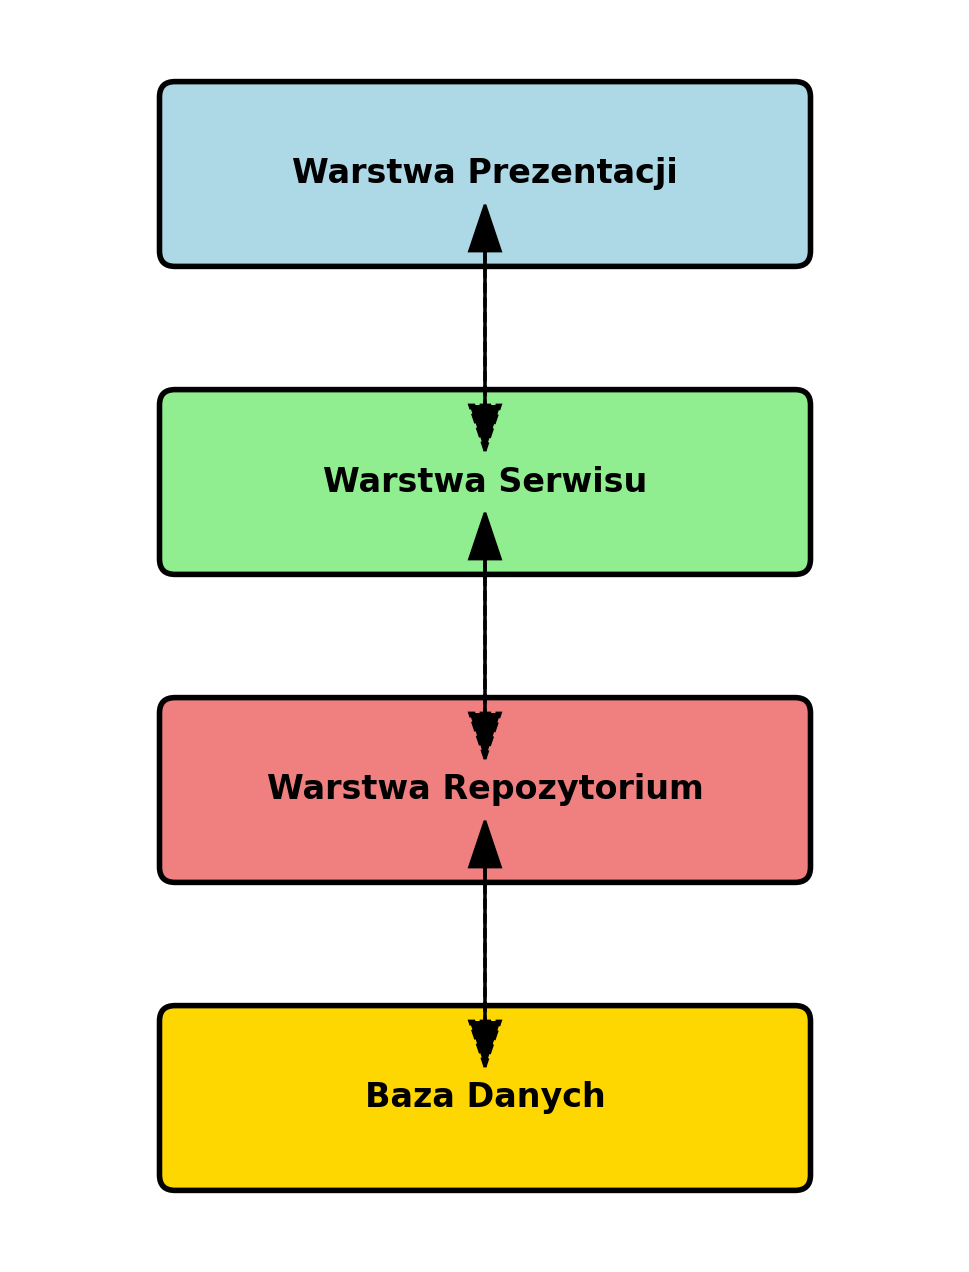
\includegraphics[width=\textwidth, height=10cm]{media/3_layer_architecture.png}

\end{center}

\subsubsection{Wrstaw prezentajcji}

Najważniejszym punktem wartstwy prezentacji w ramach logiki biznesowej było dostarczenie metod pozwalających na komunikację pomiędzy modułem obsługującym interfejs graficzny. W ramach implementacj 
programu zostały zaimplementowane cztery klasy obsługujące różnego rodzaju zapytania do serwera. Zostały one podzielone w ramach roli posiadanych przez użytkownika. Rola użtkownika w 
systemie określała jego dostęp do serwisu. W ramach aplikacji powstały 3 role (rekrut, mosowicz oraz zarząd), którym odpowiadały również kontrolery punktów komunikacji. Dodatkowo w serwisie był
kontroler obsługujący zarządnie logowania.

Przykładowa list punktów końcowychi posiadanych przez serwis:  

\begin{center}
    \begin{enumerate}
        \item localhost:8080/api/login?email=<address email zarejestorwanego użytkownika> - umożliwienie zalogowania do serwisu użytkownikowi \\
        \item localhost:8080/api/recruit/make/reservation - rezerwacja przedmiotu przez rekruta \\
        \item localhost:8080/api/recruit/equipment/list - lista dostępnych przedmiotów w kole naukowym \\
        \item localhost:8080/api/recruit/locations - lista dosępnych  lokacji w których można wypożyczyć przedmiot \\
        \item localhost:8080/api/mosowicz/make/rental - wypożyczenie przedmiotu przez członka koła \\
        \item localhost:8080/api/mosowicz/make/return - zwrócenie wypożyczonego przedmiotu \\ 
        \item localhost:8080/api/zarzad/add/item - dodanie nowego przedmiotu do wypozyczenia przez zarzad \\
    \end{enumerate}
\end{center}

\subsubsection{Warstaw serwisu}

Odpowiedzialnością warstwy serwisu jest walidacja danych otrzymanych od warstwy prezentacji oraz odpowiednie przetwarzanie oraz danych wysyłanych oraz odbieranych
od instacji warst repozytorium. Proces walidacji opiera się w głównej mierze na sprawdzaniu czy w aktualnej sesji istnieje zalogowany użytkownik, czy dane 
otrzymane w formie JSON są poprawne. Jako przykład może w tym przypadku posłużć data, która jest niezbędna do przeprowadzenia procesu rezerwacji oraz wypożyczenia.
Musi ona spełniać pewne wymagania by została ona potraktowana jako data, która jest poprawna.

Wymagania dotyczące daty początkowej oraz końcowej wypożyczenia oraz rezerwacji:
\begin{center}
    \begin{enumerate}
        \item data początkowa nie może być datą przeszłą 
        \item data końcowa nie może być datą przeszłą
        \item data końcowa nie może być datą przeszła względem daty początkowej
    \end{enumerate}
\end{center}

Warstwa serwisu została podzielona według innych kryteriów. W ramach tej warstwy został zaimplementowany serwis obsługujący logowanie, wypozyczenie, rezerwacje, 
informacji (do przeglądania informacji  o przedmiotach).

\subsubsection{Warstwa repoztyorium}

Warstaw repozytorium obsługiwala wysyłanie zaptań do bazy dancyh w celu uzyskania odpowiednich zbiorów informacji do poprawnej odpowiedzi na uzyskane zapytanie przez REST API.
W tej warstweie modelu trój-warstwowego istnieją klasy odpowiadające poszczególnym teabelom w bazie danych. Zastosowanie takiego mapowania "jeden do jeden"
względem bazy pozwala w łatwy sposób działać w ramach poszczególnych serwisów należących do warstwy powyżej. W takim przypadku każdy serwis może wywoływać zapytania do poszczególnych 
repozytoriów oraz agregować zebrane informacje w odpowiedź dla użytkownika. Natoamist instancje warstwy repozytorium mają jedną odpowiedzialność na którą składa się obsługa zapytań do
przypisanej jej bazy danych. Takie podejście jest zgodne z zasadą pojedyńczej odpowiedzialności klasy. \\

Warstawa repozytorium wykorzystuje Spring Data JPA, które ułątwia pisanie zapytań do bazy z wykorzystanie klasy EnitytManager. Pisanie zapytań z wykorzystaniem
tego modułu Spring jest znacznie prostsze w prorównaniu z pisaniem pełnych zapytań SQL w postaci obiektów typu String. 

Przykładowe zapytania napisane z wykorzystaniem Enitity Manger:
\begin{lstlisting}[language=Java, breaklines=true, caption=Przykładowy zapytanie do bazy z warstwy repozytorium, label=lst:wr]
public class EquipmentDAO {
   // ...

    @Override
    public List<ReservationRegister> findReservationsBy(UUID userID) {
        TypedQuery<ReservationRegister> query;
        query = entityManager.createQuery("FROM ReservationRegister " +
                                            "WHERE userReservation.id=:userID",
                                            ReservationRegister.class);
        query.setParameter("userID", userID);
        return query.getResultList();
    }

   // ...
}
\end{lstlisting}

Metoda findReservation wysyła zpaytanie do bazy danych w celu zwrócenia wszystkich rezerwacji dla określonego użytkownika serwisu.


\subsubsection{Klasy pomocniczne, dla modelu trójwarstwowego}

Do klas pomocnicznych dla działania serwisu trój warstwowego możemy uznać wszystkie klasy, których zadaniem było przekazywanie danych pomiędzy poszczególnymi
warstwami (DTO class) oraz mapowania tabel baz danych (Entity class).

Klasy typu DTO agregują dane wygnenerowane pomiędzy warstwami w celu przenoszenia ich. W ten sposób zostaje zachowana zasada luźnych powiązań pomiędzy klasamia.
Klasy te mogą zostać przekształcone w rekordy ze względu na fakt, że służone one jedynie do przeniesienia danych oraz ich odczytania. Nie pozwalają one na ich modyfikacje.

Klasy typu Entity są odzielnym rodzajem klas, których głównym zadaniem jest przedstawianie elementów modelu (domeny). Służą one do mapowania tabel w w ramach bazych danych.
Ich wartości mogą być zmieniane, a następnie aktualizowane w bazie danych.

\subsubsection{Testy strony serwera}

Strona serwera w głównym stopniu zostałą przetestowana z wykorzysatniem testów jednostkowych. Testy jednostkowe pokryły prawie w 100\% calą wartstwę serwisu, która jest głównym celem takich testów.
Tak wysokie pokrycie testów w przypadku warstwy serwisu wynika z faktu wykorzystania metodologi programowania Test Driven Development (TDD) stworzonej przez Robert C. Martin. Ta metodologia programowania
opiera się na pisaniu funkcjonalności, która ma zostać wprowadzona do programu. Pozwala to jednocześnie łatwo ukierunkować pracę poprzez pisanie kolejnych linii kodu oraz zapewnienienia wysokiej poprawności
napisanego kodu poprzez pokrycie go testami jednostkowymi.

Dodatkowo została przeprowadzone testy akceptacyjne, które opierały się na przetestowniu poszczególnych odowłań do REST API oraz sprawdzenia czy zachowują się one
poprawnie. Stwierdzenie czy zachowują się one poprawnie odnoście się do weryfikacji czy radzą one sobie odpowiednio zarówno z danymi poprawnymi jak i nie poprawnymi.

\end{document}
